
\subsection{分析框架}

% 根据本研究的定义,人类活动主导下的人\textendash{}水关系是社会\textendash{}水文二元循环中由人类主导的决策模式
% 而水治理(Water Governance)是指影响水使用和管理的政治、社会、经济、和行政系统相互作用的全部过程,本质上是关于``谁获得水,何时获得水,如何获得水''(``who gets water, when and how'')。
联合国开发计划署(UNDP)提出\cite{mariajacobson2013},水治理决定了与水有关的三个核心方面:``什么时候有多少水用?''``水如何为人类福祉提供不同的生态系统服务?''以及``谁能平等有效地用水?''——简而言之,水治理是决定水资源``稀缺情况''、``使用目的''、和``分配方式''的关键。
为此,本章研究将水治理的三个核心方面(``稀缺情况''、``使用目的''和``分配方式'')各自选择指标进行量化,对它们进行等权平均得到综合水治理指数(Integrated Water Governance Index, IWGI)用以识别水治理的稳态变化(图\ref{ch4:fig:framework})。
然后,通过将该指数应用在黄河这个典型的人类活动主导的流域,利用突变点检测的方法分析了$1965\sim2013$年间IWGI的变化,展示该IWGI如何有助于检测和描述复杂的水治理稳态变迁。
最后,在综合分析了水资源供需、经济发展、环境变迁,以及制度变化后,本章解释了黄河流域水治理稳态变化的主要驱动因素,并总结提出了一个过渡模式,为人类活动主导大河流域面临的治理挑战提供了抓手。

\begin{figure}[!ht]
\centering
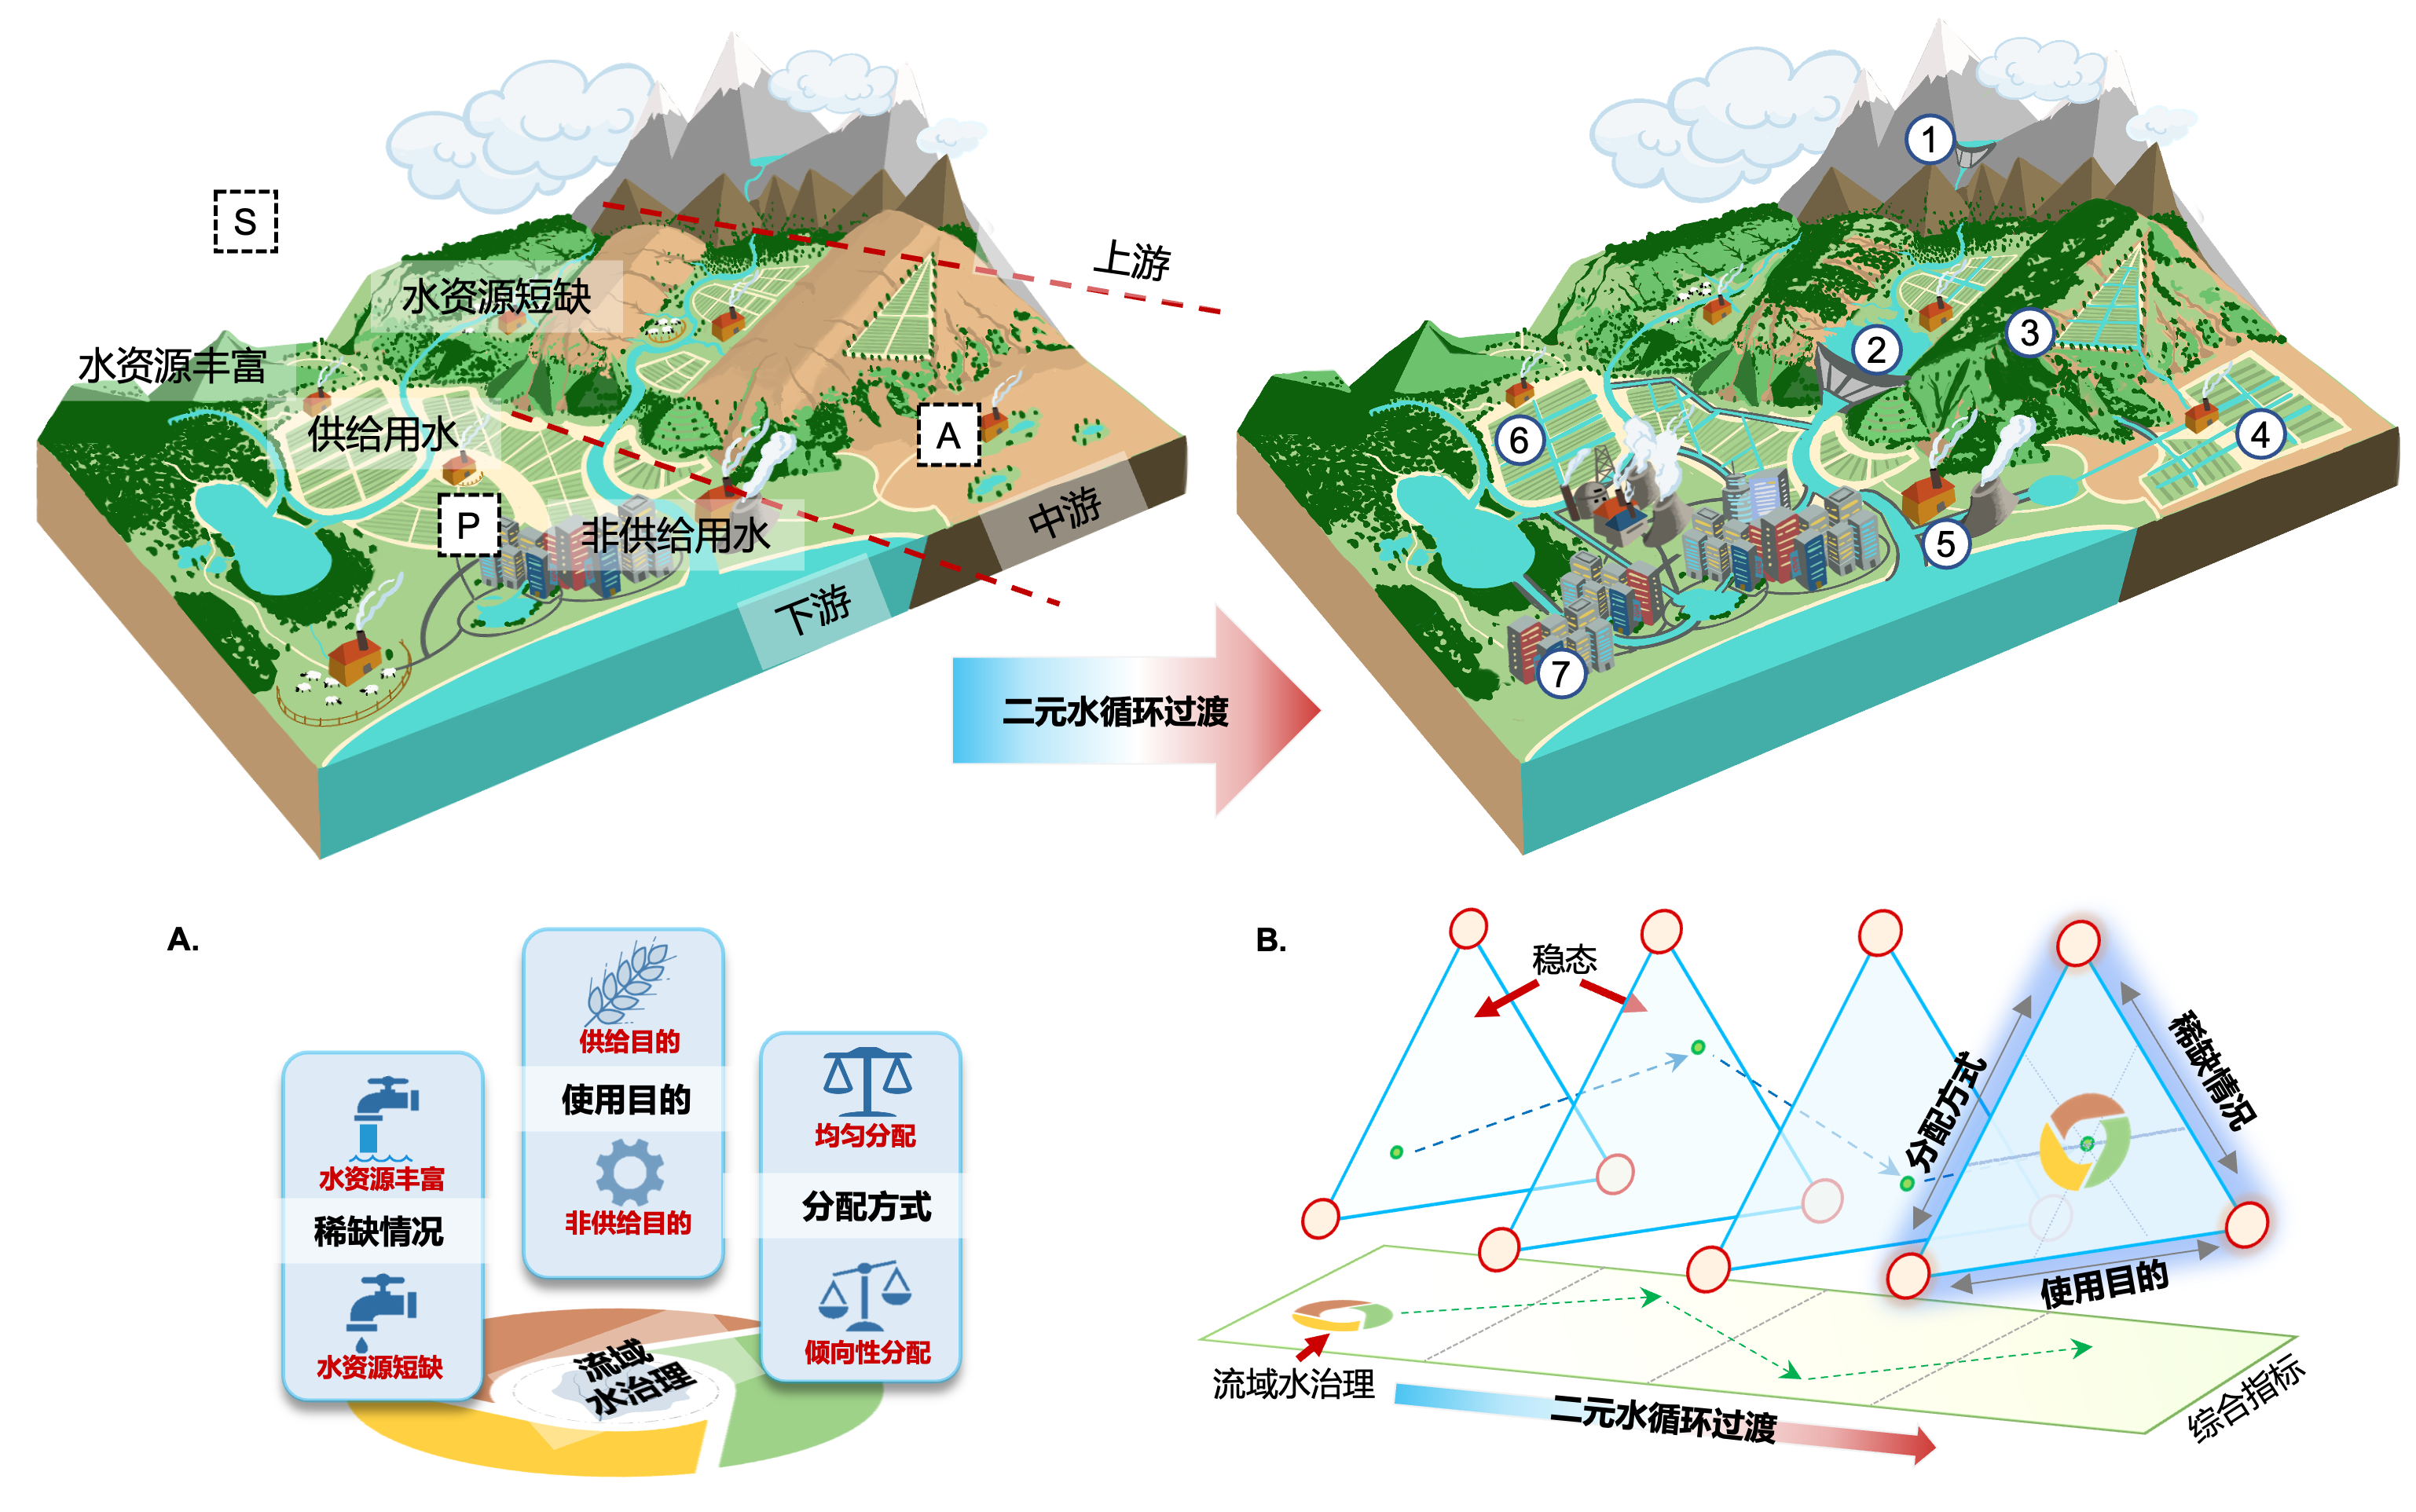
\includegraphics[width=\textwidth]{img/ch4/ch4_framework.png}
\caption[定量识别流域水治理转变的分析框架]{
    定量识别流域水治理转变的分析框架。
    \textbf{A} 利用综合水治理指数(IWGI)识别水自然\textendash{}社会二元循环过渡时期中的水治理机制,可以从稀缺情况(S)、使用目的(P)和分配方式(A)这三方面切入,三者会随着人类活动主导社会\textendash{}水文循环而变化。
    例如,水库建设(\ding{172}和\ding{173})可以缓解局地水资源压力;集约化灌溉农业的发展(\ding{174})以及能源和工业增长(\ding{175})会改变水的利用方式;输水系统控制了流域系统的水分配(\ding{176}和\ding{177})。
    \textbf{B} IWGI方法结合三个方面的相应指标,因此其突变可以指示水治理的稳态转换。}\label{ch4:fig:framework}
\end{figure}

\subsection{研究区域划分}\label{ch4:sec:region}

为便于研究的计算需要,本章参考前人研究和黄河水利委员会的标准将黄河流域划分为四个区域\cite{shuilibuhuangheshuiliweiyuanhui2010,wang2019c},以四个重要的控制水文站反映各区域的径流变化,各区域特点鲜明,便于后文对水资源治理的变化原因进行分析:

黄河源区(SR,控制水文站为唐乃亥站)人口稀少,经济欠发达,主要生态功能是水源涵养,黄河超$50\%$的天然径流来自这里。
黄河上游(UR,控制水文站为头道拐站)人均灌溉土地面积最高的区域,大量引黄河水发展灌溉农业,但灌溉效率相对较低。
黄河在中游(MR,控制水文站为花园口站)流经著名的富沙区——黄土高原,作为土壤侵蚀风险最高的地区,是黄河产沙最多的地区,近三十年的``退耕还林''生态工程显著改变了这里的土地利用覆被。
黄河下游(LR,控制水文站为利津站)人口密集,传统的农业发达地区,也曾是最大的黄河水资源使用地区。随着产业升级和节水工程的持续实施,农业用水的比重不断下降,但仍是总用水最多的地区。


% % 补充图片1:研究区示意图
% \begin{figure}[hbtp!]
% \centering
% 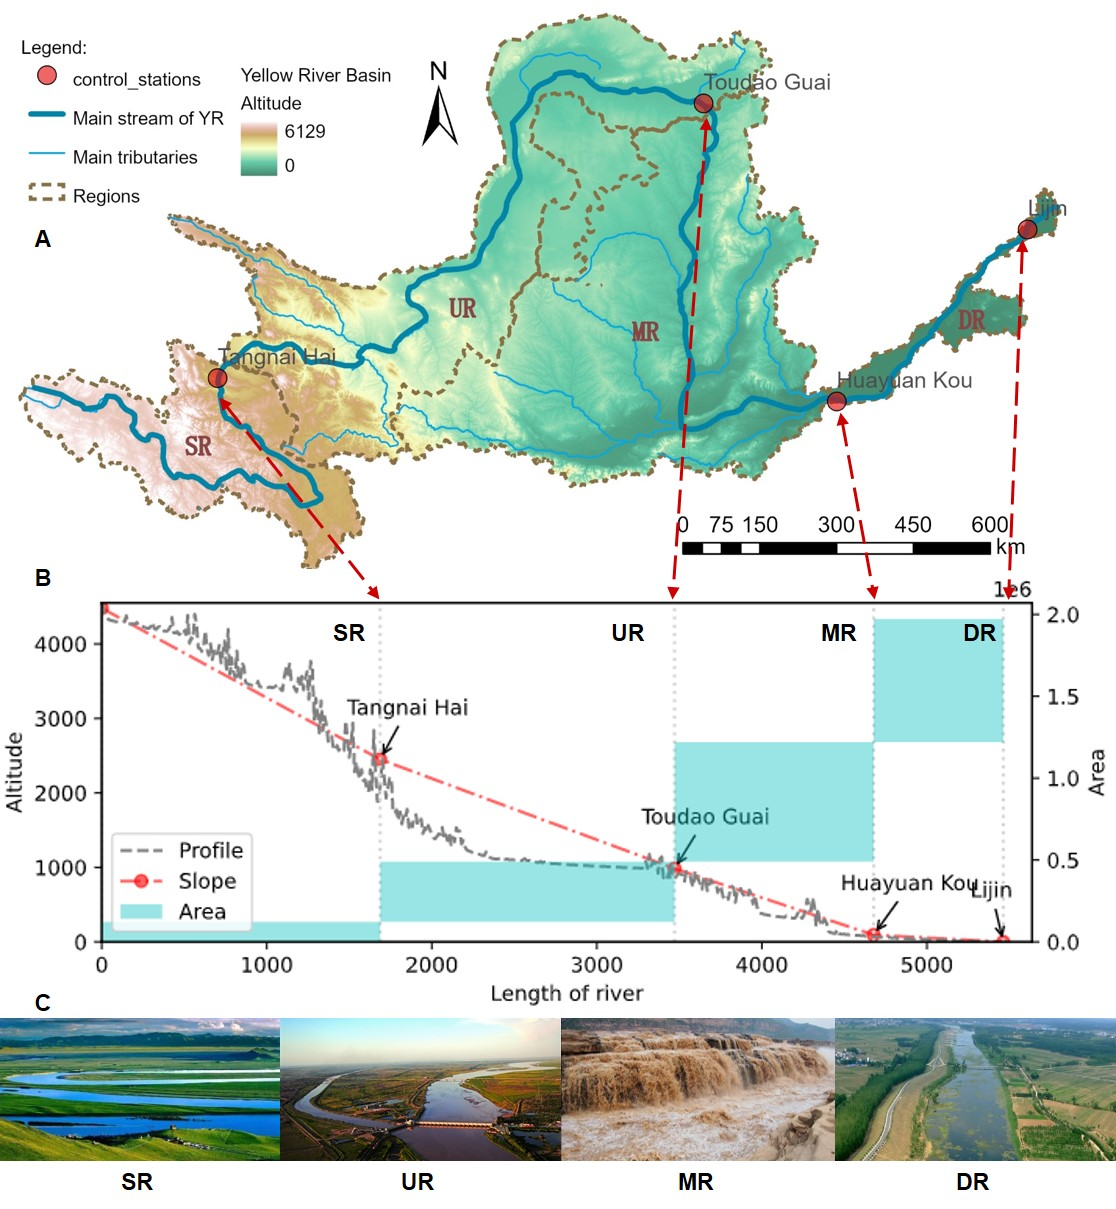
\includegraphics[width=\textwidth]{img/ch4/s1_study_area.jpg}
% \caption[黄河流域子区域划分]{黄河流域子区域划分。
%     \textbf{A.}黄河流域划分示意图(SR:源区,UR:上游,MR:中游,DR:下游);
%     \textbf{B.}黄河主河道剖面图,四个水文观测站分别控制SR、UR、MR和DR;
%     \textbf{C.}黄河流域不同地区的典型景观。}\label{fig:YRB}
% \end{figure}

\subsection{综合治理指数}

\subsubsection{综合指标构建方法}

% 将三者合一起,即:
如本章前文介绍以及框架图~\ref{ch4:fig:framework}所示,本研究定义的水资源治理综合指数(IWGI)应结合水治理的三个方面(``稀缺情况(S)''、``使用目的(P)''和``分配方式(A)'')。
由于每个指标维度都有升高和降低两个方向,在整合指标前应假设随着人类活动主导社会\textendash{}水文循环的进程,三者在其中某个方向对齐:
\begin{equation}
    Transformation \propto S*P*A
\end{equation}

接下来为三个方面选择了一个指标($I_x$, $x=S$, $P$,或$A$,分别对应``稀缺情况(S)''、``使用目的(P)''和``分配方式(A)'',来有效地量化这些方面,并将上式转化为自然对数,便于计算各指标对综合指数变化的贡献:
\begin{equation}
    Transformation \propto \ln(I_S) + \ln(I_P) + \ln(I_A)
\end{equation}
那么,综合水治理指数(IWGI)是标准化指标$I'_x$的平均值:
\begin{equation}
    IWGI = (I'_S + I'_P + I'_A) / 3
    \label{ch4:eq:IWGI}
\end{equation}
其中:
\begin{equation}
    I'_x = (I_x - I_{x, \min}) / (I_{x, \max} - I_{x, \min})
\end{equation}

对三个方面各自的指标选取如下文所述。

\subsubsection{子指标:水的稀缺情况}

水的``稀缺情况''既取决于气候能提供稀缺情况资源,还取决于灌溉和工业等经济活动的需求,更可以被水库蓄水、跨流域调水等工程所人为改变\cite{qin2019,wada2014,huang2021}。
本章研究采用Qin等人(2019)提出的稀缺性\textendash{}弹性\textendash{}易变性(SFV)水稀缺指数来评价``稀缺情况''的问题\cite{qin2019}。
这一指标考虑了管理措施(如水库的建设)和用水结构变化(有些用水方式如能源用水是难以被短期替代的),对水资源短缺情况做出评估。
此外,SFV指数从发展的角度关注水资源的动态,同时考虑了水资源的灵活性和易变性(例如气候差异带来的降水波动),是衡量水资源压力\cite{qin2019}时间变化的有效指标。
整个黄河流域的水分胁迫指标$I_S$为本章划分的四个二级区域$i$——源区(SR)、上区(UR)、中游(MR)、和下游(DR)指数$SFV_{i}$的平均值:

\begin{equation}
    I_S = \frac{1}{4} * \sum_{i=1}^4 SFV_{i}
    \label{ch4:eq:scarcity}
\end{equation}

其中$SFV_i$为区域$i$的SFV指数$SFV_i$,SFV结合了以下三个指标:

首先,对于稀缺性(Scarcity, S),$A_{i, j}$为区域$i$在第$j$年的耗水量占多年平均径流量的比例(本研究将为黄河流域划分为四个子区域,见\ref{ch4:sec:region}\nameref{ch4:sec:region}):

\begin{equation}
    A_{i, j} = \frac{WU_{i,j}}{R_{i, avg}}
\end{equation}

% TODO 完整的不灵活用水分类?
其次,对于灵活性(Flexibility, F),$F_{i, j}$是第$i$年和第$j$区域的不灵活用水$WU_{inflexible}$(例如能源行业冷却用水或人类和牲畜)占平均多年径流量的比例:

\begin{equation}
    F_{i, j} = \frac{WU_{i, j, inflexible}}{R_{i, avg}}
\end{equation}

最后,易变性(Variability, V)还考虑了水库容量和蓄水对自然径流波动的积极影响:
\begin{gather}
    C_i = C1_i * (1 - C2_i) \\
    C1_{i, j} = \frac{R_{i, std}}{R_{i, avg}} \\
    C2_{i} = \frac{RC_{i}}{R_{i, avg}}, \ if RC < R_{i, avg} \\
    C2_{i} = 1, \ if RC \geq  R_{i, avg}
\end{gather}

上式中,$R_{i, avg}$为$i$区域的平均径流量,$RC_i$为$i$区域水库的总库容,$R_{i, std}$为$i$区域径流量的标准差。

最后,该方法将三个指标(稀缺性S、灵活性F和易变性V)以相同的权重进行归一化后加权计算出$SFV$指标:

\begin{gather}
    V = \frac{A_{normalize} + B_{normalize} + C_{normalize}}{3}\\
    a = \frac{1}{V_{\max} - V_{\min}};\\
    b = \frac{1}{V_{\min} - V_{\max}} * V_{\min}\\
    SFV = a * V + b
\end{gather}


\subsubsection{子指标:水的使用目的}

水的``使用目的''与水能够提供的生态系统服务有关,但目前对文化、调节服务等缺乏成熟统一的评估框架,且受限于数据,本研究仅将用水分为供给用途(例如,日常饮用和食品生产)和非供给用途(例如能源冷却用水)的用水\cite{liu2017,florke2018,jaeger2019}。
本章研究使用供给服务目的在全部用水量中所占比例(Provisioning Purpose Shares, PPS)作为量化``使用目的(P)''$I_P$的指标。

\begin{equation}
    PPS = \frac{WU_{pro}}{WU_{pro} + WU_{non-pro}}
\label{ch4:eq:priority}
\end{equation}

其中($WU_{pro}$)为供给服务用水,包括家庭用水、灌溉用水和牲畜用水;非供给服务的用水($WU_{non-pro}$)包括工业用水和城市服务用水。
% 本章研究将牲畜用水、城乡生活用水和农业用水作为供应用水,因为它们直接服务于生存。其他的是非供应:服务和工业用水,因为它们主要为经济服务。

\subsubsection{子指标:水的分配方式}

最后,水的``分配方式''并非取决于区域的社会经济水平和自然环境背景,流域的水资源分配还会受到流域系统调度的工程(如水库统一调度)、非工程因素(如水资源分配制度)的影响\cite{schmandt2021,speed2013}。
本章借鉴使用熵作为刻画分配均匀程度的指标(式\ref{ch4:eq:allocation})\cite{peet1974},当不同区域间水资源使用完全平均时,当完全平均分配时该指标达到最大值$I_{A, \max} = 1$,当区域的用水量相差悬殊时$I_A \in [0, 1]$趋近于零。

\begin{equation}
    I_A = \sum_{i=1}^N - \log(p_{i}) * p_{i}
    \label{ch4:eq:allocation}
\end{equation}

其中$p_{i}$为区域$i$与整个流域的水量比例,由于本研究将黄河流域分为源区和上中下游,因此$N=4$。

\subsection{突变点检测}

本章研究采用Pettitt提出的的突变点检测方法,在不假设数据分布的情况下,对时间序列数据的单个变化点进行检测\cite{pettitt1979},它测试的原假设$H_0$是:变量不存在变化趋势差异,备择假设则为存在一个显著的趋势变化点。
通过将随机变量序列分为$\mathrm{x}_{1}, \mathrm{x}_{1}, \ldots, x_{t_{0}}$和$x_{t_{0}+1}, x_{t_{0}+2}, \ldots, x_{T}$表示的两段,如果每段都有一个共同的分布函数,即$F_1(x)$、$F_2(x)$和$F_1(x) \neq F_2(x)$,则在$t_0$处确定变化点。

为实现变化点的识别,定义统计指标$U_{t,T}$如下:

\begin{equation}
    U_{t, T} = \sum_{i=1}^t\sum_{j=t+1}^T sgn(X_i - X_j), 1 \leq t < T
\end{equation}

其中:
\begin{equation}
    \operatorname{sgn}(\theta)= \begin{cases}1 & \text { if } \theta>0 \\ 0 & \text { if } \theta=0 \\ -1 & \text { if } \theta<0\end{cases}
\end{equation}

找到最可能的变化点$\tau$,其值满足$K_{\tau} = \max|U_{t, T}|$,与值$K_{\tau}$相关的显著性概率近似计算为:

\begin{equation}
    p=2 \exp \left(\frac{-6 K_{\tau}^{2}}{T^{2}+T^{3}}\right)
\end{equation}

给定某个显著性水平$\alpha$,如果$p < \alpha$,则拒绝原假设并得出结论$x_{\tau}$是水平$\alpha$的显著突变点。

本章研究使用$\alpha = 0.001$作为显著性$p$的阈值,这意味着统计上显著的变化点判断有效的概率大于$99.9\%$。
迭代使用Pettitt算法:反复识别一个突变点从而将时间序列分为该时间点前后两段,并再次分别对两序列进行分析,直到检测到所有显著的突变点。
虽然接下来的结果展示的是阈值$\alpha = 0.001$的结果(识别出两个断点),但是经过敏感性分析,从$0.0005$到$0.05$的阈值范围选取都不影响本研究结果的鲁棒性(参见图\ref{ch4:fig:sensitivity})。

\begin{figure}[!ht] % use float package if you want it here
    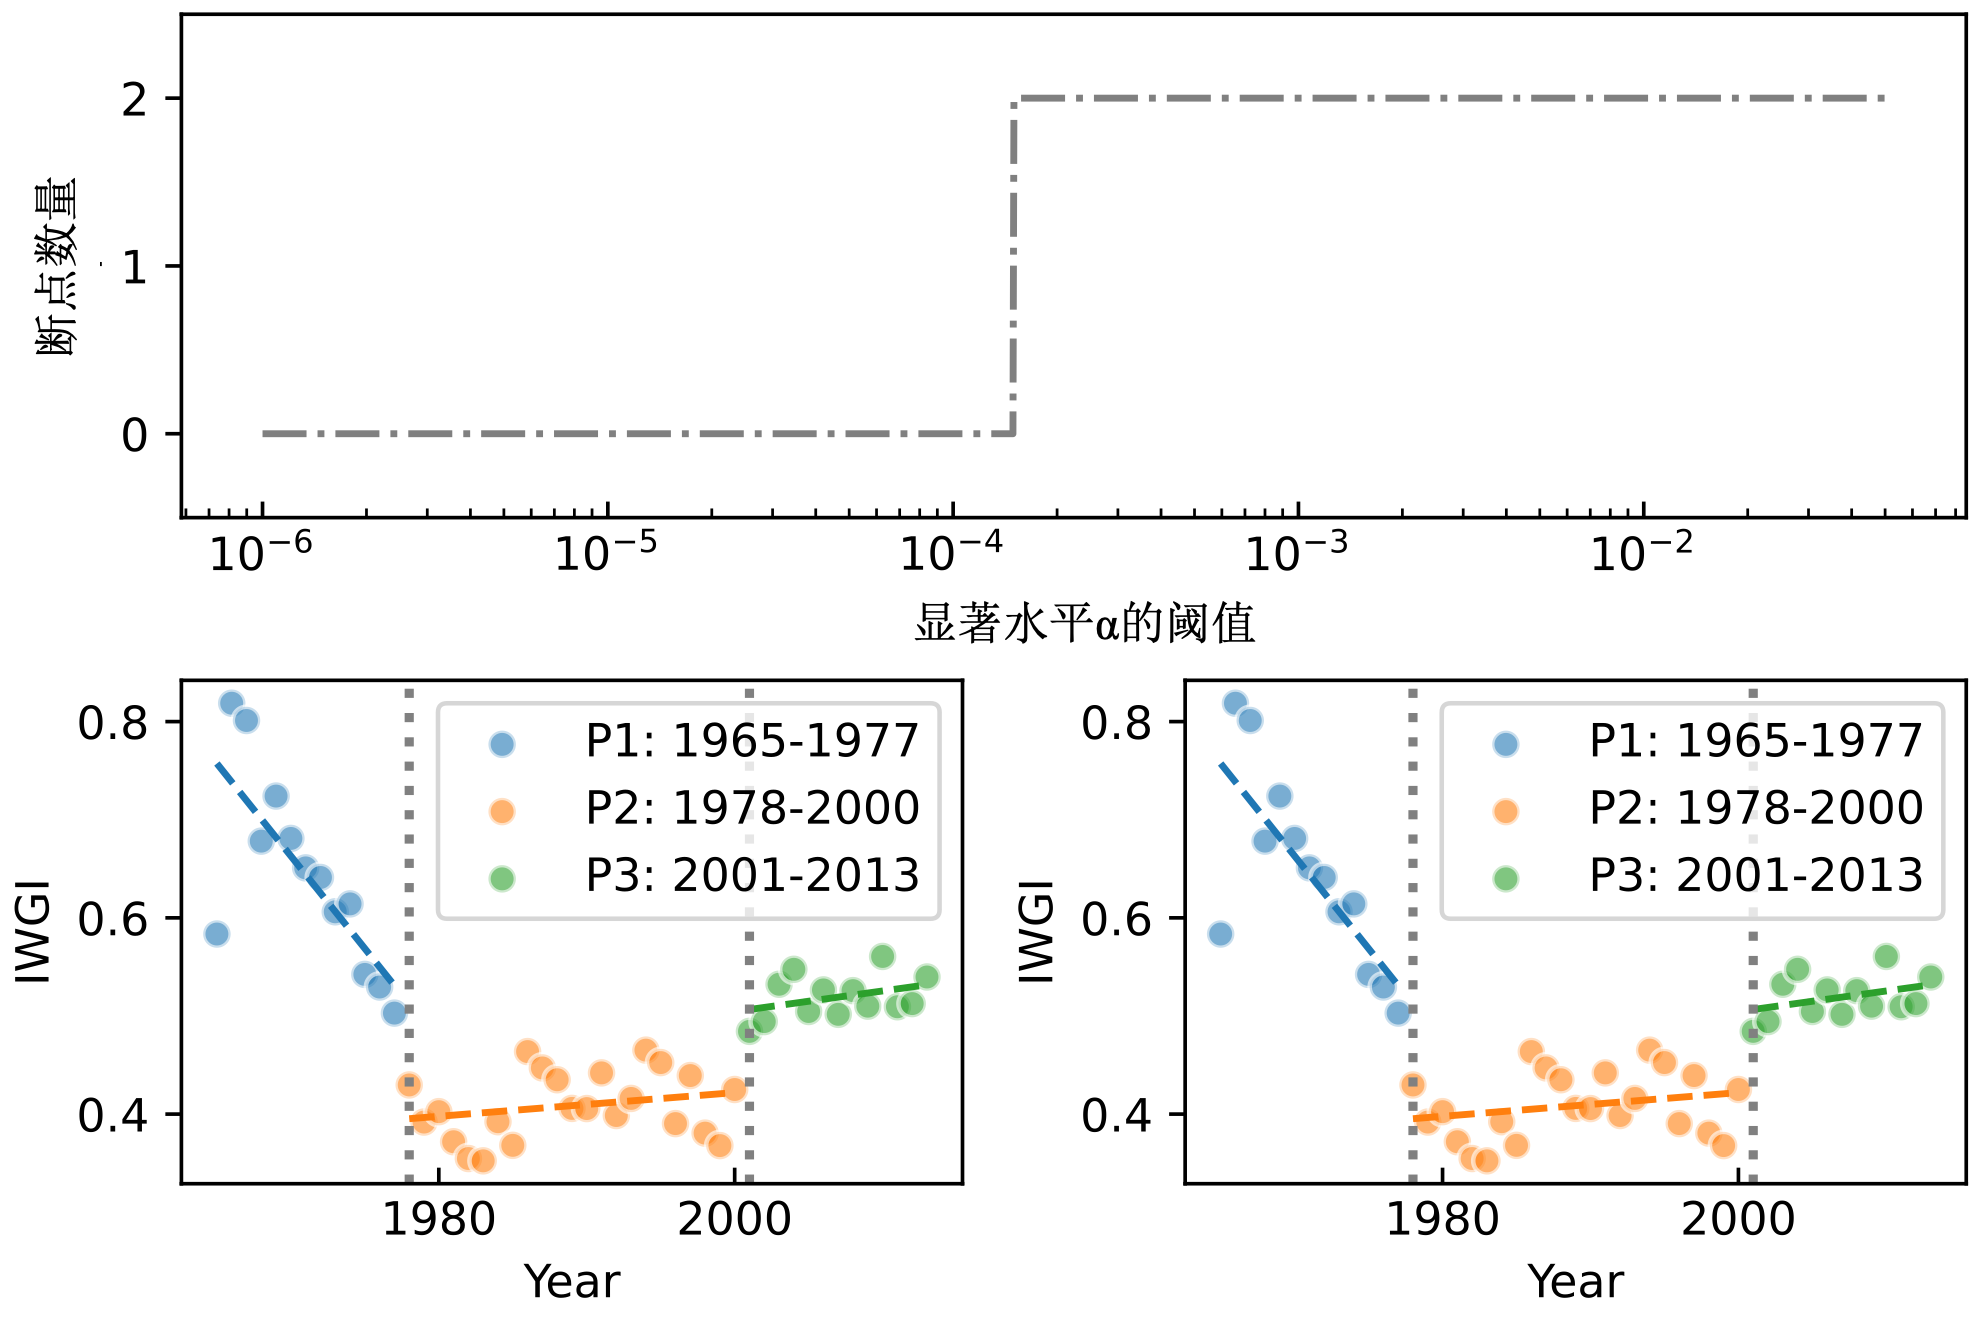
\includegraphics[width=\textwidth]{img/ch4/ch4_sensitivity.png}
    \caption[突变点检测中显著性阈值选取的敏感性测试]{突变点检测中显著性阈值选取的敏感性测试结果。
    \textbf{A} 选取不同阈值$\alpha$后识别的突变点个数,所有的方案都识别了两个断点。
    \textbf{B} 阈值选取为 $\alpha=0.0005$.
    \textbf{C} 阈值选取为 $\alpha=0.05$.}\label{ch4:fig:sensitivity}
\end{figure}

\subsection{数据来源}

% % Table generated by Excel2LaTeX from sheet '数据集'
\begin{table}[htbp]
    \centering
    \caption{数据分类与来源}
      \begin{tabularx}{\textwidth}{LLLLL}
      \toprule
      数据集   & 数据类型  & 空间尺度  & 时间尺度  & 数据来源 \\
      \midrule
      行政区水资源利用 & 统计    & 市级行政单元 & $1965-2013$ & Zhou等人2020 \\
      子流域水资源使用 & 统计    & 二级子流域 & $2003-2019$ & 水资源公报 \\
      GDP数据 & 统计    & 省级行政单元 & $1949-2019$ & 万德数据库 \\
      水库数据集 & 水文    & 站点数据  & $1949-2015$ & Wang等人2019 \\
      实测泾流量 & 水文    & 站点数据  & $1949-2019$ & Wang等人2019 \\
      黄河流域相关法律 & 文献    & 流域相关文件 & $1949-2013$ & 黄河流域规划 \\
      黄河水利委员会历史 & 文献    & 流域相关文件 & $1949-2002$ & 黄河水利委员会档案馆 \\
      黄河大事件 & 文献    & 流域相关文件 & $1949-2015$ & 黄河水利委员会档案馆 \\
      \bottomrule
      \end{tabularx}%
    \label{ch4:tab:data_source}%
\end{table}%
  

为了计算IWGI,使用了三个数据集:水库、实测径流、和用水。
水库数据集由Wang等人~\citeA{wang2019c}收集,其中包括1956年以来新建的重要水库。
在所有水库中,黄河水利委员会已经将主要用于调节和管理的水库称为``主要水库''(见\url{http://www.yrcc.gov.cn/hhyl/sngc/})。
此外,每年的实测径流数据来自《黄河泥沙公报》(\url{http://www.yrcc.gov.cn/nishagonggao/}),分别由四个控制站(唐乃亥、头道拐、花园口、利津)在黄河的不同河段(源区、上游、中游、下游)进行测量得到。
水资源利用数据来源于Zhou等人\citeA{zhou2020}发布的中国国家长期水资源利用数据集(NLWUD),包括地级市不同部门的用水量、用水经济变量和用水强度,我们以$95\%$相交面积为阈值筛选该数据集中的地级市,得到属于黄河流域的子数据集。

为了分析其变化的原因,灌溉面积、工业增加值和服务业总增加值以及用水强度数据也来自NLWUD数据集~\cite{zhou2020}。
此外,还使用了两个水治理政策数据集:法律政策和``大事件''文件数据集。
法律政策记录(表~\ref{ch4:tab:policies})来源于2013年公开批准的``黄河流域综合规划'',其中回顾了建国以来全流域尺度上的重要法律法规。
与黄河有关的``大事件''的原始文件则来自黄河水利委员会的记录和汇编(\url{http://www.yrcc.gov.cn/hhyl/hhjs/})。

本研究中使用或分析的所有数据,包括水库数据集、测量径流、用水数据集、规律和大事件,都已储存在公开获取的数据仓库中(\url{https://doi.org/10.5281/zenodo.7955500}~\cite{shuang_song_2023_7955500})。

% Table generated by Excel2LaTeX from sheet '黄河流域法律政策'
\begin{table}[htbp]
    \centering
    \caption{黄河流域法律政策}
      \begin{tabularx}{\textwidth}{L p{1.5cm} L}
      \toprule
      法律或政策名称 & \multicolumn{1}{l}{施行或修订时间} & 颁布机构 \\
      \midrule
      中华人民共和国水法 & 1,988 & 全国人民代表大会常务委员会 \\
      中华人民共和国水法  修正 & 2,002 & 全国人民代表大会常务委员会 \\
      中华人民共和国水法  第一次修订 & 2,009 & 全国人民代表大会常务委员会 \\
      中华人民共和国水法  第二次修订 & 2,016 & 全国人民代表大会常务委员会 \\
      中华人民共和国水污染防治法 & 1,984 & 全国人民代表大会常务委员会 \\
      中华人民共和国水污染防治法  修正 & 1,996 & 全国人民代表大会常务委员会 \\
      中华人民共和国水污染防治法  第一次修订 & 2,008 & 全国人民代表大会常务委员会 \\
      中华人民共和国水污染防治法  第二次修订 & 2,018 & 全国人民代表大会常务委员会 \\
      取水许可和水资源费征收管理条例 & 2,006 & 中华人民共和国国务院 \\
      取水许可和水资源费征收管理条例  第一次修订 & 2,017 & 中华人民共和国国务院 \\
      黄河水量调度条例 & 2,006 & 中华人民共和国国务院 \\
      黄河可供水量分配方案 & 1,987 & 中华人民共和国国务院 \\
      取水许可管理办法 & 2,008 & 中华人民共和国水利部 \\
      取水许可管理办法  第一次修订 & 2,015 & 中华人民共和国水利部 \\
      取水许可管理办法  第二次修订 & 2,017 & 中华人民共和国水利部 \\
      黄河水量调度条例 & 2,006 & 中华人民共和国国务院 \\
      黄河可供水量年度分配及干流水量调度方案 & 1,998 & 国家发展计划委员会,水利部 \\
      黄河水量调度管理办法 & 1,998 & 国家发展计划委员会,水利部 \\
      黄河水权转换管理实施办法 & 2,004 & 水利部 \\
      取水许可和水资源费征收管理条例 & 2,006 & 中华人民共和国国务院 \\
      取水许可证制度实施办法 & 1,993 & 中华人民共和国国务院 \\
      建设项目水资源论证管理办法 & 2,002 & 国家发展计划委员会,水利部 \\
      水利工程管理体制改革实施意见 & 2,006 & 中华人民共和国国务院 \\
      \bottomrule
      \end{tabularx}%
    \label{ch4:tab:policies}%
  \end{table}%
  

\subsection{数据分析}

\subsubsection{相关分析与显著性检验}

皮尔逊相关系数(Pearson correlation coefficient,通常用 $r$ 表示)是用于衡量两个连续变量之间线性关系强度的指标。它的值范围在 $-1$ 到 $1$ 之间,其中 $-1$ 表示完全负相关,$1$ 表示完全正相关,$0$ 表示无相关性,本研究使用该指标反映某时段内IWGI的趋势同哪些子指标变化趋势更密切,为了计算两个变量之间的皮尔逊相关系数,我们可以使用以下公式\cite{freedman2007}:

\begin{equation}
    r = \frac{\sum_{i=1}^{n}(x_i - \bar{x})(y_i - \bar{y})}{\sqrt{\sum_{i=1}^{n}{(x_i - \bar{x})}^2}\sqrt{\sum_{i=1}^{n}{(y_i - \bar{y})}^2}}
\end{equation}

其中,$x_i$ 和 $y_i$ 分别表示第 $i$ 个观察值,$\bar{x}$ 和 $\bar{y}$ 分别表示 $x$ 和 $y$ 的均值,$n$ 表示观察值的数量。计算出皮尔逊相关系数后,我们需要进行显著性检验来确定这种关系是否具有统计显著性。这里我们使用 $t$ 检验来计算显著性水平。根据 $r$ 和样本大小,我们可以计算 $t$ 值\cite{freedman2007}:

\begin{equation}
    t = \frac{r\sqrt{n-2}}{\sqrt{1-r^2}}
\end{equation}

根据统计量$t$的值查表判断显著性水平,如果 $p$ 值低于预先设定的显著性水平$0.01$,则我们可以认为两个变量之间的关系具有统计显著性。在实际应用中,我们使用 scipy 1.10.1~\cite{2020SciPy-NMeth}完成这些计算。

\subsubsection{基于平均的指标贡献度}

本研究中,表征稀缺情况的SFV指数就是稀缺性(S)、弹性(F)、易变性(V)三个指标在不同区域(源区、上游、中游、下游)之间的等权重平均(见式\ref{ch4:eq:scarcity}),综合水治理指标(IWGI)则是稀缺情况、使用目的、分配方式三个子指标取对数后的等权重平均(见式\ref{ch4:eq:IWGI})。
对此类指数,本研究中使用如下方法计算某时段某子指标($X$)对总指标变化(或指标/地区均值)的贡献度$Contribution_{X}$:

\begin{equation}
    Contribution_{X} = \Delta_{X} / \Delta_{Index}
\end{equation}

其中$\Delta_{X}$是该子指标在给定时段(从$t=start$到$t=end$)内的总变化值,$\Delta_{I}$是该子指标参与贡献的总指标总变化,两者都可以使用如下公式计算:

\begin{equation}
    \Delta=\sum_{t=start}^{end}(X_{t}-X_{t-1})
\end{equation}

上述计算方法可以计算不同时间段、不同指标的贡献度,帮助了解各指标在特定时间段内对总体变化的影响程度。

\subsubsection{基于比例的指标贡献度}

本研究中供给性用水比例(表征使用目的,见式\ref{ch4:eq:priority})以除法形式进行计算,在分解各部门用水对比例变化的贡献时应取对数:

\begin{equation}
    \log{(\text{ratio})}=\log{\frac{A}{B}} = \log{A} - \log{B}
    \label{ch4:eq:log}
\end{equation}

本章感兴趣的是在时段开始($start$)到结束($end$)之间 $C$、$A$ 和 $B$ 的变化,我们可以将 C 的变化量表示为 A 和 B 变化量的加权和:

\begin{equation}
    \begin{aligned}
    & \Delta \log (C)=\log \left(C_{end}\right)-\log \left(C_{start}\right) \\
    & \Delta \log (A)=\log \left(A_{end}\right)-\log \left(A_{start}\right) \\
    & \Delta \log (B)=\log \left(B_{end}\right)-\log \left(B_{start}\right) \\
    & \Delta \log (C)=k_1 \cdot \Delta \log (A)+k_2 \cdot \Delta \log (B)
    \end{aligned}
\end{equation}

结合式\ref{ch4:eq:log},可以得到A 和 B 分别对 C 变化的贡献比例 $k_1$ 和 $k_2$:

\begin{equation}
    \begin{gathered}
    k_1=\frac{\Delta \log (C)}{\Delta \log (A)} \\
    k_2=\frac{\Delta \log (C)-\Delta \log (A)}{-\Delta \log (B)}
    \end{gathered}
\end{equation}
